\documentclass{report}
\usepackage{natbib}
\usepackage{geometry}
\usepackage{pdfpages}
\usepackage{gensymb}
\usepackage{todonotes}
\usepackage{listings}
\usepackage[titletoc]{appendix}

\geometry{a4paper, portrait, margin=1in}

\begin{document}

% \includepdf[pages={1}]{data-mining-coversheet.pdf}
% \setcounter{page}{1}

\title{Dissertation} \author{Oliver Marshall}
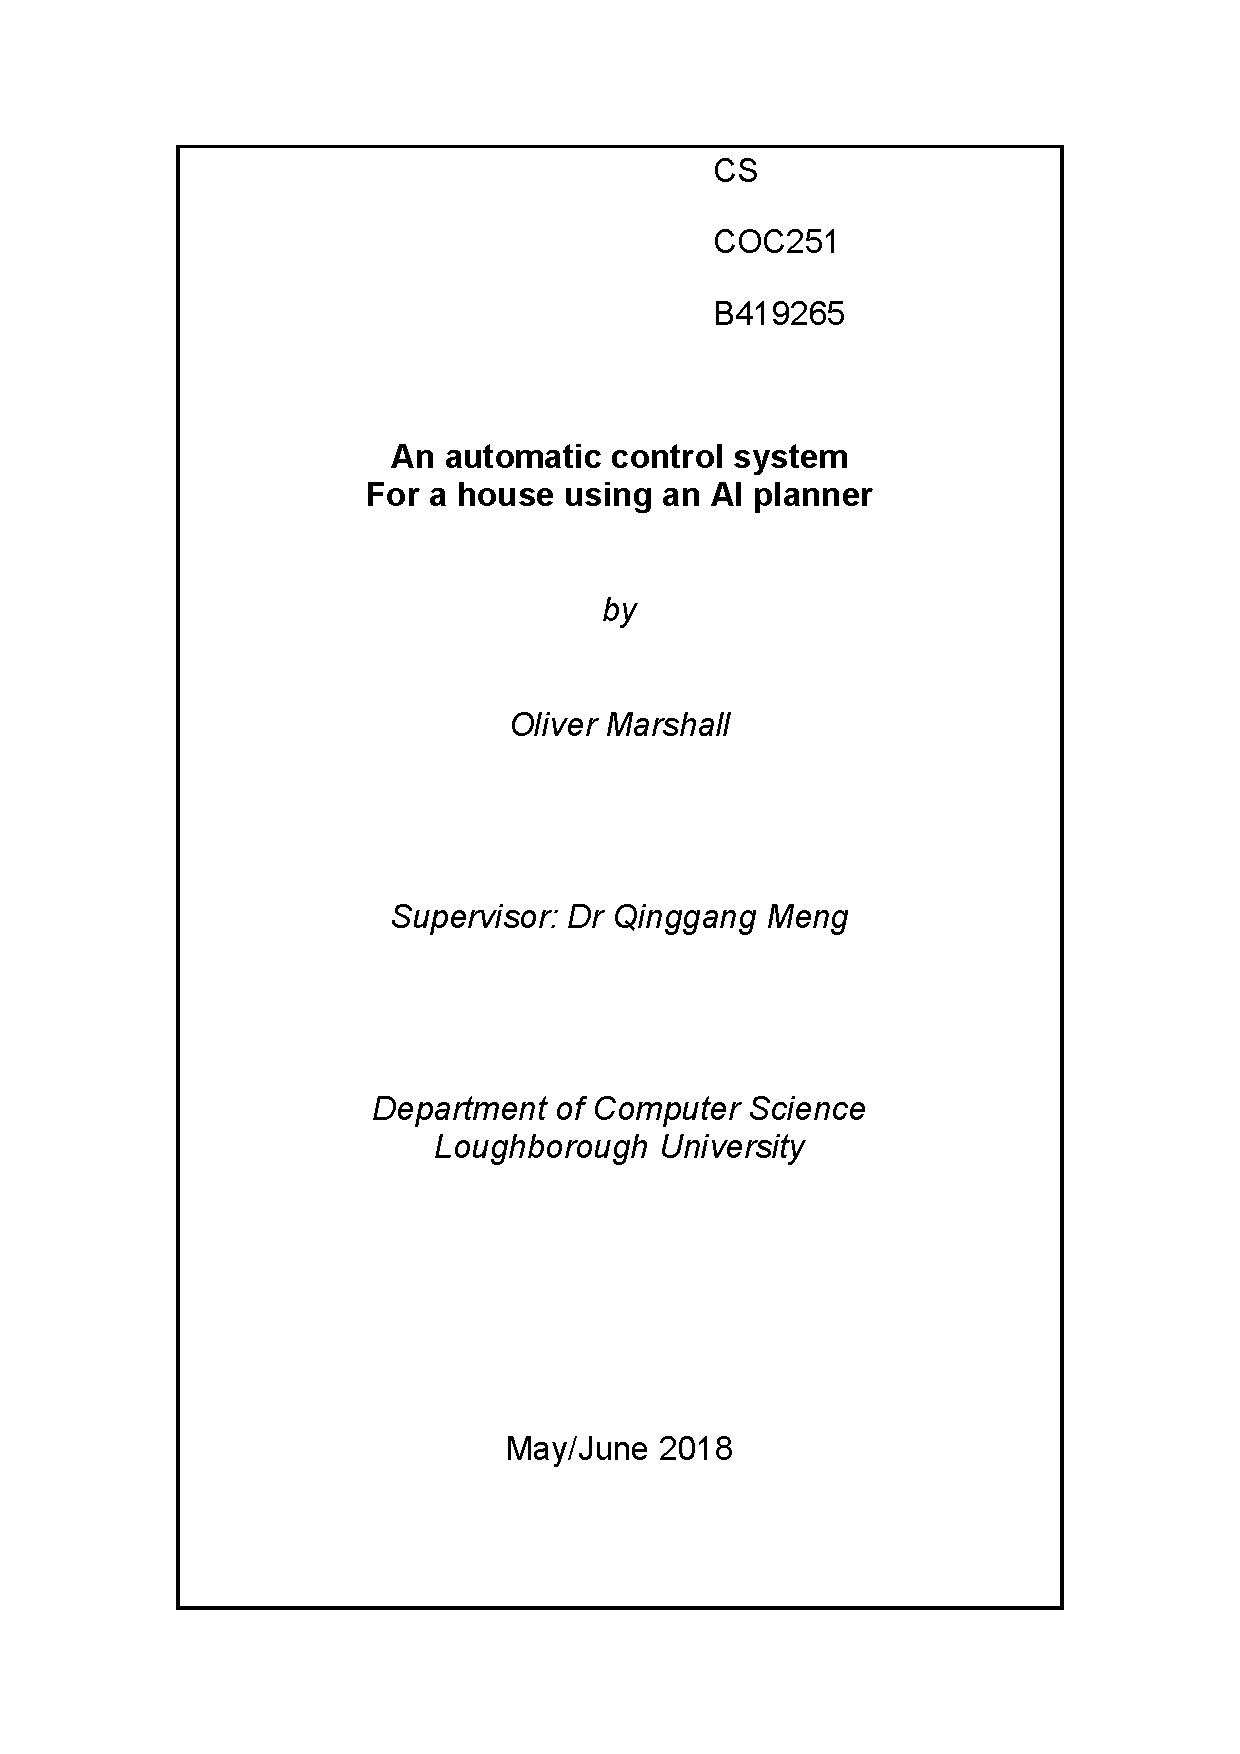
\includepdf{fyp-coversheet.pdf}
\newpage

\begin{abstract}
  In this document I describe and implement the core of a home automation system
  which uses a Hierarchical Task Network planner to plan actions that the
  automation system should take. The core accepts as input a set of user defined
  `domain extension' files as well as a `problem' file that are combined
  together to form a more complete understanding of the context of the problem.
  Allowing third parties to define the domain extensions enables the easy
  extension of the home automation system to work with new devices.

  This document starts by introducing the problem to be explored in the rest of
  the document, this is followed by a literature review investigating the
  current approaches to home automation and automated planning. It then details
  the design, implementation and testing of the core of a home automation
  system. Finally it concludes by discussing the achievements of the system as
  well as additions to the system to improve the design.
\end{abstract}
\newpage

\renewcommand{\abstractname}{Acknowledgments}
\begin{abstract}
  I would like to acknowledge the help and encouragement offered by me project
  supervisor, Dr Qinggang Meng. His help pushed me to create a better solution
  that I could have otherwise.
\end{abstract}
\newpage

\tableofcontents
\newpage

\listoffigures
\newpage

\chapter{Introduction}
In 2010 it was estimated that nearly 12.5 billion devices were connected to the
internet, and it was predicted that by 2020 that number could increase to 50
billion devices \citep{Evans2011}. As the number of internet enabled devices
grows it becomes increasingly likely that these devices will end up in the
average home. This increase in the number of devices and number of interactions
a user will likely have with these devices produces two main problems: how to
effectively manage the devices; and how to allow multiple devices to interact.
These problems can be solved by introducing `control software' which allows the
user to configure how they want the devices in the system to interact with each
other as well as to solve problems and follow any rules they give it.

The most commonly used of such software is software provided by the
manufacturer, that way the user has some guarantee that the software will work
with the devices they own. An issue with this is that the manufacturer has
different goals to the user which can lead to problems such as old devices
ceasing to work on newer software, and devices from other manufacturers not
working with the software at all. Another issue with most device control
software is that it is difficult or impossible to extend to add new or custom
devices with unique behaviors that can interact with the rest of the system
fully.

A solution to this problem could be to have a core system that can be extended
by software written by third parties. This could allow users to develop their
own solutions to devices not working in their system and share their solutions
with other users.

In this document I will show my research into the extent to which current
control software supports extension and investigate the current approaches to
automated planning and how this can help with enabling the extension of home
automation software. I will then design and implement a solution that can
demonstrate how effectiveness automated planning is as a solution to this
problem.

%%% Local Variables:
%%% mode: latex
%%% TeX-master: "../diss"
%%% End:

\chapter{Literature Review}
\section{Internet of Things}
``The Internet of things is the network of physical devices, vehicles, home
appliances and other items embedded with electronics, software, sensors,
actuators, and network connectivity which enables these objects to connect and
exchange data \citep{Contributors2018}". This year it is estimated that there
are over 20 billion IoT devices connected to the internet \citep{Statista2015}
with predictions that there will be up to 50 billion devices in 2020
\citep{Evans2011}. With this increasing number of devices inevitably a large
portion of these devices end up in home environments. For these devices to
produce a useful output there needs to be some intelligence managing and
controlling them. This could be the user manually controlling the devices, the
devices communicating with and controlling the other devices in the network or
via a central intelligent controller. The latter is what I will be focusing on.

\section{Home Automation}
In the review of home automation systems done by \cite{Lobaccaro2016}, it can be
observed that most of the systems reviewed are either closed source systems or
do not support a large range of devices. Extensibility is an important feature
of home automation as users won't always want to be locked into using a specific
set of devices when they choose a controller for their home automation system.
An avenue that hasn't been considered is using automated planning to control the
devices, by using a domain-independent or domain configurable device new actions
could be added by the devices as they enter the system, or the controller could
detect new devices and add actions accordingly.

\section{Automated Planning}
The Handbook of Knowledge Representation defines automated planning as "the
deliberation process that chooses and organizes actions by anticipating their
expected effects" \citep{Cimatti2008}.

\section{Classical planning}
Classical planning is an active area of research concerning planning, but the
key point of this area is that it constrains the planners by making a series of
assumptions that limit the types of problems that can be solved by the planners.
These assumptions mainly concern things that usually affect real- world systems
such as implicit time taken or sequential plans. Because of this, most problems
that are likely to be faced when using planning in the real-world are unable to
be solved by a purely classical planner. And as classical planning is the main
focus for much of the research done in planning these assumptions have effects
on other planners developed outside of classical planning.

\section{Domain specific}
This area of planning relies on encoding domain information into the planner
itself, allowing the planner to make efficient plans to solve problems in this
domain. The downside of this type of planner is that it is locked into the
domain of problems it attempts to solve, and cannot be used in other domains
without major work being done on it.

\section{Domain independent}
This is the type of planner that has been the focus of the most research as
classical planning comes under this topic. This style of planning focuses on
making the planning algorithm able to solve problems from different domains,
they do this by having the actions available be part of the input to the
planner. By doing this they are more flexible than domain-specific planners as
they can solve problems for many different domains instead of just one, but
because the domain-specific planner can encode information about the domain,
domain independent planners tend to have worse performance.

\section{Domain configurable} \label{section:domain-configurable}
A middle ground between domain-specific and independent planners is domain
configurable planners, these can solve a wide range of problems well and quickly
as shown in the International Planning Competition in 2000 and 2002, and they do
this without having to program a new core. They do this by allowing domain
information to be encoded in the problem definition allowing the planners to
decrease the search space and thus decrease search time and enabling them to
produce better plans. There are two main types of configurable planning:
hierarchical task network (HTN) planner, which plans by decomposing tasks into
subtasks continually until only primitive tasks remain; and control-rule
planners which define a set of rules for invalid states allowing the planner to
backtrack until a new valid path is found. Benefits of these planners include:
having a mobile core like domain-independent planners which reduces the amount
of work needing to be done to introduce a new problem to the planner; by having
knowledge about the domain, the planner can produce better plans faster.

\section{Comparison}
\cite{Nau2007} compares these different types of planners using three different
comparisons: upfront effort, performance and coverage. In his comparison he
found that configurable planners performed well compared to the other planners,
having lower upfront costs than domain-specific planners but higher than domain
independent, but by they also performed better than domain-independent planners
although worse than domain-specific planners although he did note that "a
sufficiently capable domain-configurable planner should have nearly the same
level of performance because it should be possible to encode the same
domain-specific problem-solving techniques into the domain description". In the
author's research into the International Planning Competition, he found that
domain configurable planners end up having better coverage than the other types,
the author contributes this "partly to efficiency and partly to expressive
power". From this comparison, configurable planners seem to be the best choice,
especially if you are going to be solving different problems like in home
automation.

\section{Conclusion}
The area of home automation is already large and will be growing every year,
because of this it is important that the control systems we develop are easily
extensible and smart enough to solve the increasing demands of the system's
users. Domain configurable planning seems to be a good way of solving this
configurability problem as it can solve problems from many different domains
while still remaining performant. Planning's applicability to this domain has
not been explored before, this might present some problems, but these should
have been explored when applying planning to other domains, so they should be
easy to overcome. Something I have not seen any research on is the effectiveness
of extending a domain via plugins provided by multiple parties, this is
something I plan to base a large part of my project on.

%%% Local Variables:
%%% mode: latex
%%% TeX-master: "../diss"
%%% End:

\chapter{Design}
Home automation software brings together two things: devices, and user defined
rules. They do this to provide a service to control and manage the devices
according to the user defined rules.

\section{Devices}
Devices can be either a physical product for example a smart light or another
piece of software for example an email client. Both physical and software
devices need to have some way to be controlled by the home automation software,
for this it is obviously necessary that either: the devices themselves send a
message to the home automation software to tell it their capabilities; the
automation software `scans' for devices somehow; or a third party system sends a
message instead that does the same.

\subsection{Devices Support My System}
One advantage of this type of design is that my system can be `device agnostic'
which means that if a manufacturer decides to add a new feature to a device or
come out with an entirely new type of device, then my system does not have to be
updated. This helps to keep the maintenance cost of my system down as I would
not need to be continually updating my software as new devices come out. As well
as allowing for device manufacturers to update their products to add new
features without having to worry that my system will support it.

Another advantage to this design is that it also allows the manufacturers to be
in control of what actions can be performed and how which can allow them to tune
the device to work better with my system and so provide a better product. This
has a disadvantage tied to it though as it gives manufacturers control over the
types of actions that can be performed, because of this there may be types of
actions that the manufacturer did not consider that the user's system then
wouldn't be able to perform. Manufacturers could also choose to not support
features that they know the next version of the device will be able to perform
to help convince users to buy the newest product instead of updating the old
one.

A disadvantage of this design is that it limits the devices that can connect
with my system to only those that support my system, manufacturers that want to
push their own home automation systems would simply not support my system and
older devices would not be supported as manufacturers would rather users bought
newer products instead of spending money to update the older versions.

Another disadvantage of this design is that devices would have to be continually
supported by the manufacturer, which is a cost for them that they would rather
avoid. This is mitigated by the fact that the manufacturers would already have
to be supporting the product, but this does add another cost of support staff
training and maintenance costs.

\subsection{My System `Scans' For Devices}
This type of design has the advantage that devices manufacturers would not have
to support or even know about my software for my software to support their
devices. This lowers the costs for manufacturers but increases the development
and support costs for my software greatly.

This design would have high development costs due to the large number of devices
that would need to be supported and that most devices would require reverse
engineering which is both costly and time consuming. Reverse engineering has the
added detriment that the manufacturer could change how the devices works
internally which could make my system either stop working completely or falsely
assume that the devices is working fine.

The system would require frequent updates as new devices come out, this could
mean that users have to update their automation software even though the devices
they are using haven't change or been update.

\subsection{Third Parties Add Support For Devices}
\label{section:third-party}
This type of design is similar to the devices themselves supporting my system
and allows my system to be `device agnostic'. By instead allowing third parties
to add support for new devices as well as update devices more devices can have
support added quickly by community members via `plugins' to my control system.
This also helps reduces the support cost of my software as the developer of the
plugin would provides support and updates to the plugin themselves.

As development of plugins would be a community effort lots of effort would have
to be put into standards and conventions for plugin development, if this was not
done then it would be easy for plugins to become incompatible with each other as
they could use slightly different terminology to refer to the same thing, for
example the `afternoon' could be referred to as `lunchtime' in other plugins
which would confuse users and other plugin developers.

An advantageous example of a convention that could emerges would be `middleware'
which is when similar devices are grouped together under the same group of
actions. For example there are many manufacturers of smart lights, if a user has
more that one in their home automation system then it could cause confusion
about what `actions' to use to control which type smart of smart light.
Middleware could group these different types of smart lights under a set of
actions that would work with all of them which provides a consistent interface
for the user to interact with.

By allowing anyone to develop these plugins it would be easy for users to add
support for their own DIY projects. Many of these DIY projects would be unique
or specific to their circumstances so if either of the other designs were chosen
then it would be either costly if difficult to support them. Another advantage
to allowing anyone to develop plugins is that they might be able to come up with
ideas for devices of actions for existing devices that manufacturers and other
users would not have thought of before.

The disadvantage of allowing third parties to develop plugins is that they don't
always have the time or money to support the plugins that they write, this can
lead to plugins being abandoned by the original developer. This doesn't have to
be a large issue though because as long as the device doesn't change too much
after the plugin is abandoned the plugin could still work with the device. It is
also possible for other developers interested in the device working in their own
homes could start supporting the old plugin.

An disadvantage to allowing anyone to develop plugins is that the quality of the
plugin isn't guaranteed, so the plugin could be written by someone who doesn't
know the conventions or the plugin could have bugs that could interfere with
other plugins or even stop the automation process entirely. This could be fixed
by having a repository of plugins that have been verified to work well with the
device and other plugins.

\section{Rules}
User defined rules are an important part of a home automation system as without
them the system wouldn't do anything. Rule systems on other home automation
systems tend to have a simple system for defining rules that allows users to
define a condition whether an action or group of actions takes place or not. A
smarter system would allow the user to combine these conditions to allow more
freedom and flexibility. This is the essence of how the automated planning
method Hierarchical Task Network (HTN) works. A list, called the task list, of
`methods' and `operators' is provided to the planner which then decomposes the
methods into either methods or operators until only operators remain, at this
point a `plan' is formed and can be executed. When these methods are decomposed
preconditions are checked to select which methods or operators to decompose the
parent method into, this allows for a more flexible way of defining rules.

There are many other types of planners but an HTN planner was selected for this
project because, as specified in section \ref{section:domain-configurable}, it
is a domain configurable planner. This allows the rules for the planner (also
know as the domain) to be specified separately to the planner which is useful
for this project because the rules for each user will be different depending on
their needs and what devices they have.

\section{Identifying of Groups of Users}
A key area to consider when designing software is to think about who the users
of the end system will be. In the case of my project I have identified three
groups of users who would interact, each group has different requirements from
my system and so should be considered in the design.

\subsection{The End Users}
This group of users are the users that actually interact with the various
devices and rules configured in the system. They only interact with devices
controlled by the system and have no interaction with the control software at
all. Because of this the responsibility for the design decisions for this type
of user can passed onto the other types of users. All that needs to be done is
to make sure that the other types of users produce designs that this group of
users can use easily, this can be helped by producing a set of guidelines or
standards to follow that will help the system run smoothly. This is only an
appropriate design decision because part of the expected goals of managers and
developers is for the system to work well for the end users which is aligned
with my goal as the system designer.

\subsection{The Managers}
The managers are the group of users that add new devices to the system as well
as configure the rules for the system to follow. Users in this group are not
expected to have a detailed knowledge of the system and so are only expected to
interact with the system via a high level user interface, that I expect to be
developed `on top' of the system I will design. This type of user wants to be
able to easily setup new devices to work with the system, to be able to setup
rules for the system and it's devices to follow as well as being able to be able
to tell what will effect the configured rules will have. The rules these
managers create will need to interact with the devices configured in the system.
How these devices can be interacted with is defined by the developers, this can
have some benefits, for example as described in section
\ref{section:third-party} `middleware' can be used to abstract away unnecessary
details for the managers such as the different kinds of lights that might exist
in their system.

\subsection{The Developers}
The developers is the group of users I will be focusing on the most while I am
designing my system as they will be interacting with the system directly,
whereas the other groups of users interact with my system indirectly via user
interfaces or by interacting with the devices themselves. I expect this group to
consist mainly of community members who own the device they are developing the
software for, the benefit for them being that their device will then be capable
of working with the rest of the system, it is also possible for the
manufacturers of devices themselves to put out an `official' plugin for my
system as well which would allow them to increase the amount of users that would
want to buy their product. These plugins would be shared via some kind of
`repository' system, this would allow users to select which drivers they want to
install in their home system. Because of this only one developer would need to
write software for a particular device to allow anyone else who wishes to use
that type of device with my system would be able to just by installing the
plugin. This group is expected to interact with my system by writing software
`plugins', these plugins can fall into two categories: drivers and middleware. A
driver is a piece of software that provides my system with a list of actions
that the device can perform along with information on how the action will affect
the state of the world. Drivers also provide a way for the control system to
tell the device to execute the action. Middleware builds on top of drivers to
provide more complex functionality by composing multiple actions together in
different ways. This allows the developers to provide more consistent actions
for managers to work with, as well as allowing them to add additional features
to the devices by combining together actions.

\section{Core Design}
For this project I will only be focusing on the design of the `core' of this
project, because of this I will consider designing the UI for the managers out
of scope, but I will consider how they will provide the rules for the system.

The core of this system will consist of an automated planner, which will be
provided by an external program, along with a wrapper around the planner that
collects together the inputs to the system into appropriate forms for the
planner and then formats the output of the planner. An external planner was
chosen because a planner is a complex system on it's own that would be a full
research project.

The type of planner my design will use is a Hierarchical Task Network (HTN)
planner. This type of planner as discussed in section
\ref{section:domain-configurable} is a domain configurable planner meaning that
the inputs provided to it to produce a plan are a `domain' and a `problem'. An
HTN planner was chosen because this type of planner allows information about the
environment to be included in the input to the planner, this is important
because if this weren't the case then information about devices would have to be
included in the planner itself which would mean that the plugins described in
section \ref{section:third-party} would be impossible.

The ability to specify domain information externally to the planner has another
benefit in that this information can be provided in multiple parts and then
combined together into a single `domain' to be input into the planner. This is
what my system will do, developers will provide drivers and middleware in the
form of `domain extensions' that give information on how actions affect the
state of the world, and managers will provide a set of rules for the system to
follow in the form of a domain extension and a problem. These domain extensions
and the problem will then be used as inputs to my system which will combine
together the extension to form a complete domain description for the system and
a problem description that can be used as the input to the external planner.
This process is shown in figure \ref{fig:domain-diagram}.

\begin{figure}
  \centering
  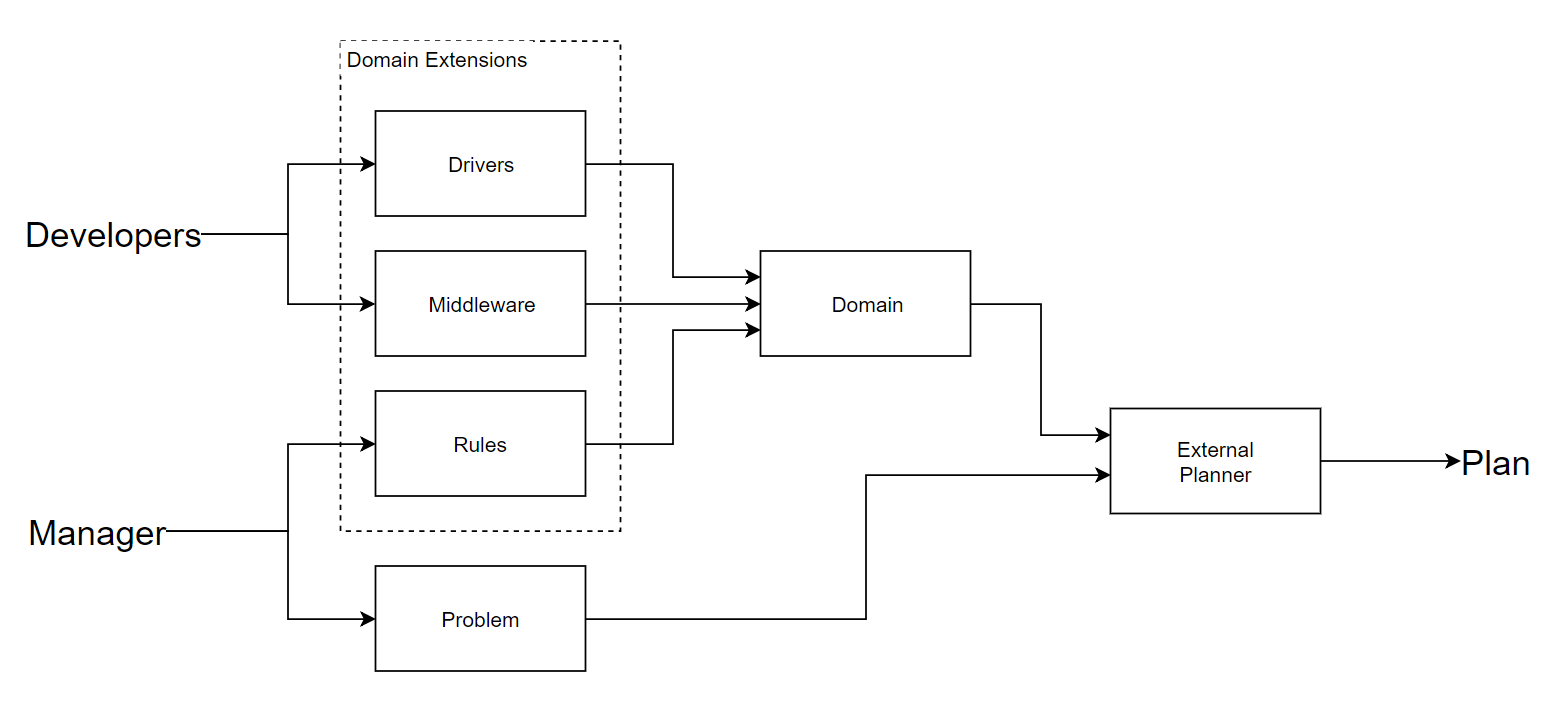
\includegraphics[width=1\linewidth]{figures/domain-diagram.png}
  \caption{The flow of data structures through the core of the design}
  \label{fig:domain-diagram}
\end{figure}

As mentioned in the previously, managers will provide rules via domain
extensions. This is because these rules are descriptions of how the manager
want's the domain to work as oppose to a description of a problem. The managers
also supply a problem to be solved, this is in the form of a list of tasks to
take, these will usually be the `rules' specified by the manager in the earlier
step. The problem also includes information about the current state of the
system, this would have to be provided by the developers when writing their
plugins as an `initial state' of the device.

Once the domain and problem have been collected by my system and transformed
into a form that the external planner can process, my system will execute the
external planner to work out a plan. The planner must be able to output whether
a plan has been found or not as well as being able to output the lowest cost
plan that has been found.

\section{Plan Execution}
Once the core has found a plan it is ready to be executed. The external planner
can provide facilities to plan for multiple tasks to be run at the same time to
reduce the amount of time taken for a plan to complete. The plan generated would
be passed out to the home automation system to be executed in the order given,
but this step is omitted as I am only designing the core.

After the plan is executed the core starts another round of planning, in my
simple design my core does not receive feedback on the execution of the plan
because this would greatly increase the complexity of the design. I will go into
greater detail as to why this is in section \ref{section:flaws}, but for this
specific case I would have to introduce a new type of devices called a `sensor'
which would give information about the state of the world to the system. The
largest issue of adding these sensors is the form in which they provide
information the system would have to be standardized with the devices which
provides a large amount to additional complexity to the conventions that would
have to be designed for them.

\section{Flaws}
\label{section:flaws}
In his work \cite{Nau2007} describes a conceptual model for a planner (I have
included this in appendix \ref{appendix:dynamic-planning}). As part of his
description of domain-independent planning he also describes a set of assumption
that restrict the domains that classical planners can work on (I have included
these assumptions in appendix \ref{appendix:assumptions}), these assumptions can
also be seen as restrictions on classical planners that don't allow them to work
on problems in the real world without heavy amounts of abstraction between the
problem and the planner. Although the HTN is not a classical planner all of
these same restrictions apply to the design that I have laid out.

\paragraph*{\textit{Restriction R0 (Finite $\sum$).}} HTN planners are not
designed around a system of states in the same way that classical planners are,
but there does exist a function that can transform HTN's internal representation
of state to be the same as that of a classical planner. What this restriction
means for HTN planners is that there can exist states that the planner cannot
express, so therefore there can exist plans that it is impossible for the
planner to account for. This does not limit the planner too much as the domain
tends to have encoded in it enough information to produce states which are
useful to it.

\paragraph*{\textit{Restriction R1 (Fully Observable $\sum$).}} Because my
design does not incorporate the use of `sensors' it has no knowledge of events
this means that the planner's state-transition function will be incomplete
meaning that it cannot react to external stimulus or unexpected consequences of
actions. My design also assumes that developers are able to accurately predict
all the consequences of the actions the devices can take. The consequence of
this restriction is that the system will be inaccurate, although it is
impossible to say how inaccurate and what effect the inaccuracy would have on a
real example would be without testing the system.

\paragraph*{\textit{Restriction R2 (Deterministic $\sum$).}} My system assumes
this to be the case in many places: it does not account for errors in tasks and
assumes they will always produces the same effect on the state of the system; or
it does not account for the possibility of devices having a random factor in
them which can be useful in some cases, for example a system to output a random
fact of the day. This is a restriction that it is hard to overcome as the system
due to the nature of the restriction.

\paragraph*{\textit{Restriction R3 (Static $\sum$).}} My system currently does
not support events due to the fact that it does not support sensors and that
devices have no way of communicating the execution status of the actions have
been performed. This has drastic effects on the usefulness of the planner as
this means that it cannot react to external stimulus, this means that the users
can have no input to the system. This restriction would be solved by adding
support for sensors in my system, but this has been deemed out of scope.

\paragraph*{\textit{Restriction R4 (Attainment Goals).}} This kind of
restriction means that it is impossible to restrict the system to no visit
certain states in the plan. This means that if the system was required to adhere
to safety restriction it would be impossible to do so with the current design.
This could be remedied by building in safety restrictions, but because I would
not be the one building the plugins to the system it would be impossible to
enforce as developers could fairly easily get around any restrictions.

\paragraph*{\textit{Restriction R5 (Sequential Plans).}} The consequence of this
restriction is that certain types of plans will be inefficient or too slow to be
useful for the user. This can be easily remedied by changing the external
planner to one that allows asynchronous planning.

\paragraph*{\textit{Restriction R6 (Implicit Time).}} This restriction is no
easy to fix because as \cite{Nau2007} states `This assumption is embedded in the
state-transition model, which does not represent time explicitly'. This can be
partially fixed by introducing a cost parameter to actions and events in the
planner, this would allow the system to avoid actions that cost a lot either in
time or resources.

\paragraph*{\textit{Restriction R7 (Off-line Planning).}} This restriction can
mean that plans get outdated while they are still being created. In the
environment of a home automation system, the speed of events and actions is
expected to be relatively slow compared to how quickly the planner can create
new plans because of this, this restriction should not effect the system too
much.

\paragraph*{}
The aim of this project is not to address these restrictions, so most of these
are deemed to be out of scope in the design, but for a next version of this
design these would need to be considered as they have great effects on the
design.

%%% Local Variables:
%%% mode: latex
%%% TeX-master: "../diss"
%%% End:


\chapter{Implementation}
\section{Selecting an External Planner}
As discussed in my design I will be creating a wrapper around an existing
external planner to collect together domain extensions and a problem to use as
input to the planner. SHOP2 (Simple Hierarchical Ordered Planner) is a
domain-independent automated planner, and the JSHOP2 (see appendix
\ref{appendix:JSHOP2}) implementation has great documentation (see reference
\cite{Ilghami2006}) as well as being free and open source is the perfect
external planner for my needs. Because it is a domain-independent planner it
accepts inputs of the domain and problem which describe the problem to solve as
well as the context (or domain) in which it should be solved. JSHOP2 expects
these input to be expressed in it's own planning domain definition language,
this is useful because I can modify the syntax of this language to allow for
domain extensions while still keeping the expressive power of the language.
Using JSHOP2's domain language also has the benefit of making it easier to
transform from my modified version to the version that JSHOP2 can process with
few errors.

\section{Parsing and Encoding}
The first part of my core design is to read domain extension and a problem
specifications supplied by the user. For this I needed to specify a domain and
problem language, luckily JSHOP2's documentation \citep{Ilghami2006} includes a
full definition of the data structures that make up domain language. To parse
the domain language and then encode it into a form that the JSHOP2 planner would
recognize I wrote three modules of code: a parser to initial parse and verify
that the domain extensions and problem are of the correct form; a pre-compiler
to process the representation produced by the parser into an internal
representation that is easier to work with; and an encoder which takes the
internal representation for the domain-extensions and parser and produces the
domain language that JSHOP2 recognizes.

\subsection{Parser}
Because SHOP2's original implementation is written in lisp, JSHOP2's domain
language takes heavy influence from lisp. This ends up being very useful when
parsing the language because I chose to implement the JSHOP2, wrapper in a lisp
family language called `Clojure' (see appendix \ref{appendix:clojure}). What
this means is, to read the domain extensions and problems I can just use the
`read-string' function provided by the language. By using functions included in
the language itself I can even get the added benefit of ignoring comments which
is a feature present in JSHOP2's specification with no extra effort.

To parse the domain-extensions and problem I used a Clojure library called
`clojure.spec' (see appendix \ref{appendix:clojure-spec}), this library allows
you to specify how a piece of data should be structured and any predicates that
the should be true for the data. This ends up being very similar to how JSHOP2's
documentation describes the domain language, because of this the parser is very
similar to the original JSHOP2 documentation.

\subsubsection{Differences to JSHOP2}
While writing the parser for the domain language I introduced a few minor
differences to the domain language to help increase readability of the language.
I have detailed these below:

\begin{itemize}
\item The `assign' keyword used for assignment is now `def', this is more
  similar to how clojure defines variables.
\item Task lists are vectors instead of list, this means that they use square
  brackets `[,]' instead of ordinary brackets `(,)'. This helps to differentiate
  them as a data structure.
\item Delete lists and add lists are also vectors.
\item Conjunctions now \emph{must} begin with an `and' keyword, unless they
  contain no expressions in which case they may be an empty list. This helps to
  distinguish between lists and conjunctions even further.
\item There is no way to specify a `domain', instead a vector of `axioms',
  `operators' and `methods' must be specified as a domain extension. These
  domain extensions will later be combined to form a single domain.
\item A problem does not specify what domain it will use as it is assumed that
  the domain will be the one created by merging the domain extensions.
\end{itemize}

\subsection{Pre-compiler}
The parser validates that the domain extensions and problem is of the correct
form, but it does not produce an output that is not easy to process. Because of
this a pre-compiler is needed to process the output of the parser into a form
that is easy to then encode into the form that JSHOP2 can understand. The
internal representation is similar in structure to how the language is defined,
each form stores information related to itself and it's children, but doesn't
store anything related to it's parent. The internal representation is defined
using a clojure data structure called a `record', this record is a map of keys
and values with some extra properties that allow for groups of functions call
`protocols' to quickly dispatch (choose the correct function to call) on.

\subsection{Encoder}
Because the internal representation is a nested structure of records (which can
be thought of as typed map or dictionaries in other languages), this allows me
to write the encoder in a way so that each records `knows' how to encode itself
using a protocol and can just recursively call the encode function on each of
it's children, if any, to build up it's encoded version. Because of this
property it was very easy to write the encoder part of the core, as I just had
to know how each type component in the domain language was expressed in JSHOP2's
language and write that out as a quoted form then finally serialize the newly
converted domain and problems into files for use in the external planner.

\section{Wrapping JSHOP2}
JSHOP2's planning process has 3 main stages to it: compiling the domain and
problem; recompiling the problem file; and finally running the problem to find a
plan. To properly `wrap' JSHOP2 I had to be able to execute this functionality
and read the results from within the core of my design.

\subsection{Calling JSHOP2}
Clojure is a language that runs on the Java Virtual Machine (JVM), this allows
clojure to offer interoperability with java code. I used this `interop' to call
the function that compiles the domain and problem files inputting the files
generated in the previous steps.

\subsection{Recompiling the Problem File}
JSHOP2 compiles it's domain and problem files into java source code that needs
to be compiled before it can be run, this requires that the java compiler be run
with the files produced by the previous step as inputs. The easiest way to do
this I found was to use the clojure library `clojure.shell' (see appendix
\ref{appendix:clojure-shell}) which allows me to make calls to the command line
of the operating system. Using clojure.shell I simply called the java compiler
`javac' to compile the problem file as specified in JSHOP2's documentation.

\subsection{Parsing JSHOP2's Output}
Once the problem file has been compiled it can simply be run using the
clojure.shell library and executing the compiled java files. The planners output
simply contains a line stating whether any plans were found or not, and if a
plan was found then it states a task list that would solve the problem specified
and a cost for the plan. These are simply parsed as strings and printed to the
user.

\begin{figure}
  \centering
  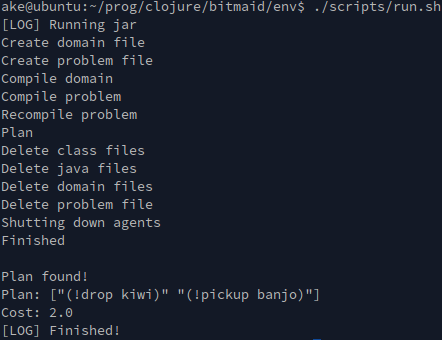
\includegraphics[width=0.6\linewidth]{figures/core-output.png}
  \caption{An example of a simple domain and problem being solved using the core
    and external planner.}
  \label{fig:core-example-output}
\end{figure}

%%% Local Variables:
%%% mode: latex
%%% TeX-master: "../diss"
%%% End:

\chapter{System Testing}
Because clojure is a dynamic language and a lisp it is usual to test the system
while writing the functions by using the REPL. In the case of this project this
was not enough because each component in the system was large and interconnected
to itself. Because of this I wrote tests covering each section.

\section{Parser - 320 assertions}
\label{section:parser-testing}
This component was the section that I focused most of my time testing on. This
is due to the fact that it is the only component that interfaces with input from
the user, user input can be of any form so it is effective to spend more effort
on places in the code that have to deal with it.

Because when I was developing the parser I had documentation that explained in
detail the domain language (see \cite{Ilghami2006}), it is was easy to test that
each of the different expressions worked as it was supposed to. Also, due to the
recursive nature of the language, I could test each expression individually to
check that it was working properly and then trust for the tests following it
that that expression would parse as expected.


\section{Pre-compiler - 147 assertions}
\label{section:pre-compiler-testing}
As I did not expect the parser to handle every case perfectly the next most
important place to test was the pre-compiler. This ended up being very useful as
a few errors did make it past the parser that I had not found. These errors
usually ended up being me misunderstanding how the clojure.spec library worked
and so I will not go into them here.

It was also useful to test that the data structures had the correct types of
children attached to them and that each of the properties attached to the data
structure was correctly filled.

\section{Encoder - 37 assertions}
\label{section:encoder-testing}
The encoder was the last component in the core that I built, and so it the
component that I spent the least time testing. What is important about testing
this component though is that this is the first time that a full end-to-end test
could be done. Because of this most of the tests in this section are tautologies
as most expressions are not expected to change too much as they pass through the
system.

\section{End to End test}
\label{section:end-to-end}
As a final test for the system I put together a simple example of a house with
several light in it. In this example the user has setup two rules: if it's the
afternoon and any of the lights are on then turn off all the lights; and if it's
either the morning or the evening and any of the lights are off then turn all
the lights on. This example is included in the `example/' directory in the base
of the source-code folder as well as in appendix \ref{appendix:home-example}.

The example is made up of several files, the problem file `p.prob' contains
information about the current state of the system, i.e. there are several
lights, some of them are on and some are not, and the hour of the day is 12.
There are three domain files the first of note is the `user-rules.dext' file,
this file is expected to be automatically generated by a user interface that the
manager of the automation system would configure.

The second file to look at would be the `time.dext' file, this extension is an
example of added functionality that could be provided by middleware as it
provides a series of axioms that use the `hour' predicate to provided a more
useful measure of time.

The third and final file is `light1.dext' which is the domain extension written
as a `driver' for the lights in the house. It is expected that this file would
be written by a third party and imported as part of a `plugin' package. This
file defines a series of operators which define the actions that the device as
well as the plugin can perform.

The results of this test is that a plan is formed to turn off all the lights as
the `afternoon' predicate is true and some of the lights are on, if the hour is
changed in the problem description file then the outcome of the test changes.
This the expected outcome of the test and shows that multiple domain extensions
can be combined together to perform a single task.

\begin{figure}
  \centering
  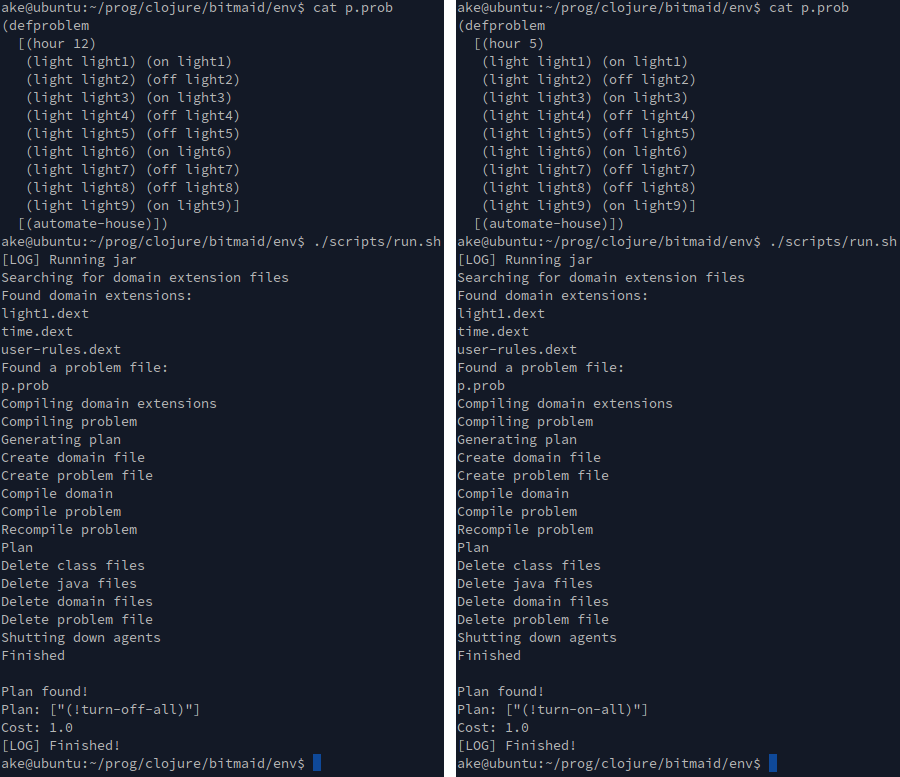
\includegraphics[width=1\linewidth]{figures/house-example.png}
  \caption{An example run of a simple example (a) with the hour set to 12 and
    (b) with the hour set to 5.}
  \label{fig:house-example}
\end{figure}

%%% Local Variables:
%%% mode: latex
%%% TeX-master: "../diss"
%%% End:

\chapter{Conclusion}
In my work I have described the design of a system that allows users to define
`domain extensions' as a way of combining disparate information about a domain.
This method of combining knowledge provided the advantage of allowing multiple
different third parties to write software that integrated well with the rest of
the system. By allowing multiple third parties to develop software for the
system the software can grow quickly as users discover devices that they wish to
be integrated in the system. Because the software plugins developed by these
third parties is separate to the system I have designed, the core that I have
designed is not effected by the development of these plugins which means that my
system remains easy to maintain no matter the number of devices integrated.

This method also has some disadvantages in that if the third parties are writing
software about similar devices or concepts, then an agreement needs to be made
about the terms used and their meaning in context with the system, if this is
not done then it can be easy for the system to develop complex hard to fix bugs.
A resistance against this could be to have an official `repository' of plugins
that have been compared to a set of standards to reduces the number of such
collisions. This solution introduces extra maintenance costs as well as
possibly stifling the growth of plugins that work differently to how the
standards might expect.

This project has shown that this method is feasible at least in small cases,
more work would need to be done to show it working in larger test cases. Work
has also not been done to address the feedback required for the state of the
world to change nor has work been done to address concerns of actions taking a
real amount of time.

Overall I think this project has successfully implemented a core of a home
automation system. I think more work should be done on the home automation
surrounding my core design and there are many interesting problems still to be
solved surrounding this solution.

%%% Local Variables:
%%% mode: latex
%%% TeX-master: "../diss"
%%% End:

\begin{appendices}
  \chapter{Tools Used}
  \section{JSHOP2}
\label{appendix:JSHOP2}
From the SHOP project homepage \citep{UniversityofMaryland2006}:

\begin{quote}
  Our most recent planner is JSHOP2, a Java implementation of SHOP2 (which is
  written in Lisp). In addition to being in Java, JSHOP2 uses a new planner
  compilation technique to synthesize domain-dependent planners from SHOP2
  domain descriptions. This way, JSHOP2 can do a variety of optimizations to
  speed up execution.
\end{quote}

\section{Clojure}
\label{appendix:clojure}
From the Clojure.org homepage \citep{Hickey2018a}:

\begin{quote}
  Clojure is a dynamic, general-purpose programming language, combining the
  approachability and interactive development of a scripting language with an
  efficient and robust infrastructure for multithreaded programming. Clojure is
  a compiled language, yet remains completely dynamic - every feature supported
  by Clojure is supported at runtime. Clojure provides easy access to the Java
  frameworks, with optional type hints and type inference, to ensure that calls
  to Java can avoid reflection.

  Clojure is a dialect of Lisp, and shares with Lisp the code-as-data philosophy
  and a powerful macro system. Clojure is predominantly a functional programming
  language, and features a rich set of immutable, persistent data structures.
  When mutable state is needed, Clojure offers a software transactional memory
  system and reactive Agent system that ensure clean, correct, multithreaded
  designs.
\end{quote}

\section{Leiningen}
\label{appendix:leiningen}
Leiningen is one of the most widely used build tools for clojure. It's use is to
create and manage projects written in the clojure language as well as providing
tools and plugins to aid in development.

\section{Clojure Spec}
\label{appendix:clojure-spec}
From the GitHub page \citep{Hickey2018}:

\begin{quote}
  spec is a Clojure library to describe the structure of data and functions.
  Specs can be used to validate data, conform (destructure) data, explain
  invalid data, generate examples that conform to the specs, and automatically
  use generative testing to test functions.
\end{quote}

\section{Clojure Shell}
\label{appendix:clojure-shell}
Clojure.shell is a library that allows the programmer to pass calls to the
command line of the operating system. This can give them access to external
programs that they would not otherwise be able to access.

%%% Local Variables:
%%% mode: latex
%%% TeX-master: "../diss"
%%% End:

  \chapter{Conceptual Model for Planning}
  \label{appendix:dynamic-planning}
  \begin{figure}
  \centering
  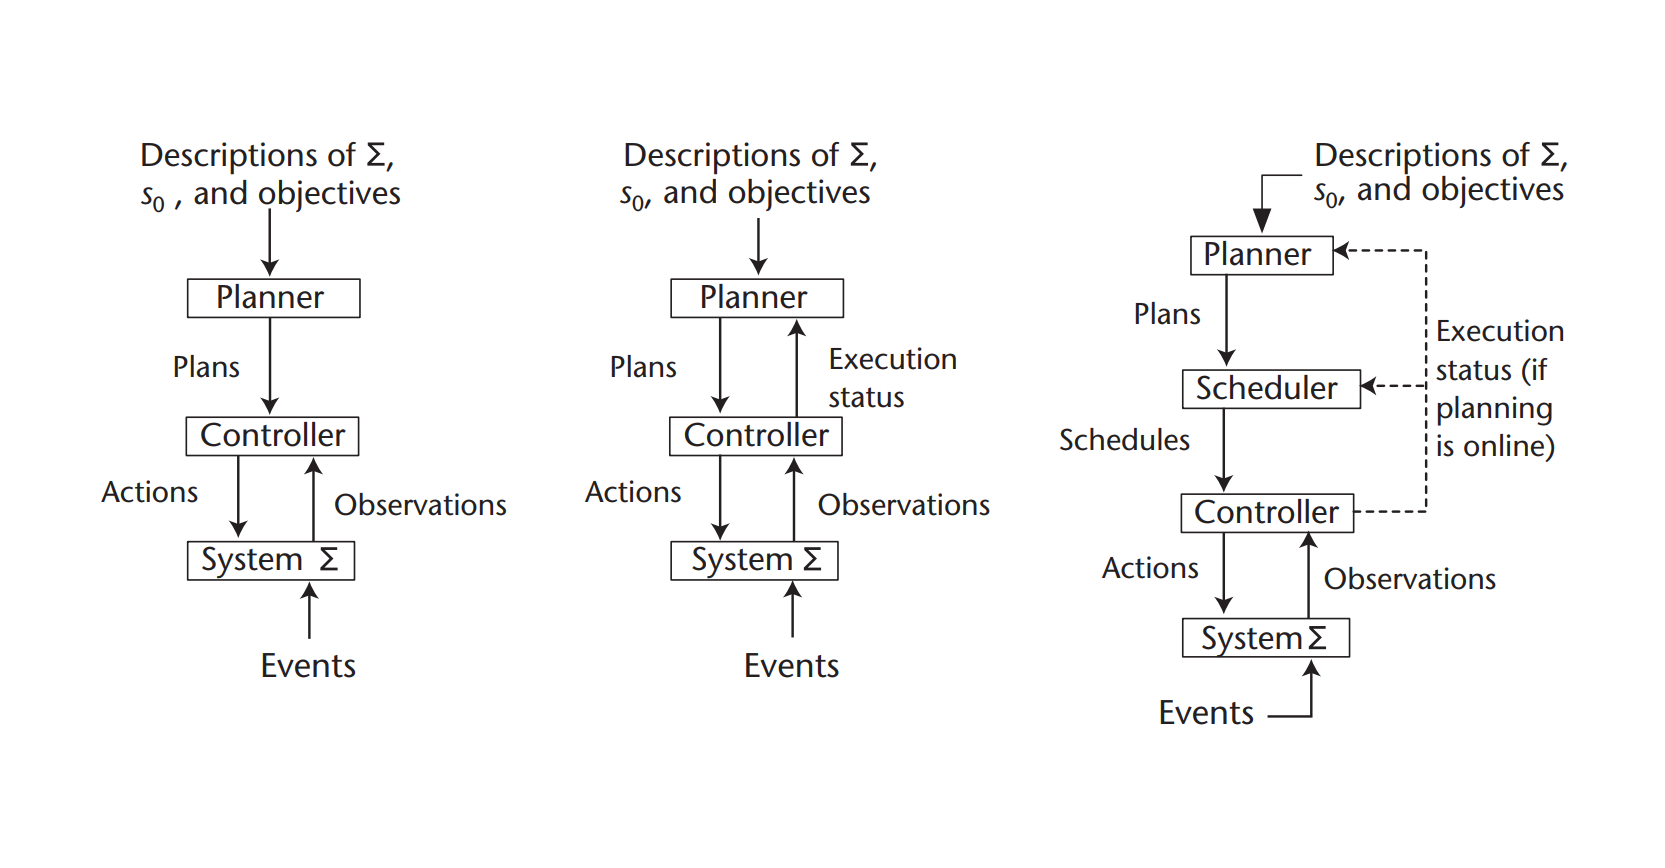
\includegraphics[width=1\linewidth]{figures/planner-diagram.png}
  \caption{Simple Conceptual Models for (a) Offline Planning, (b) Online
    Planning, and (c) Planning with a Separate Scheduler.}
  \label{fig:planner-diagram}
\end{figure}

\newenvironment{sspara}
  {\begin{quote}
    \sffamily
  }
  {
    \normalfont
   \end{quote}
  }

This chapter has been included in verbatim from \cite{Nau2007}'s work describing
the current trends in automated planning. It is included to help give context to
the assumptions at the end of this section which I have used as examples of
restrictions to the planning model. In his work \cite{Nau2007} describes a
conceptual model for planning as the following:

\section{Conceptual Model for Planning}
A conceptual model is a simple theoretical device for describing the main
elements of a problem. It may fail to address several of the practical details
but still can be very useful for getting a basic understanding of the problem.
In this article, I'll use a conceptual model for planning that includes three
primary parts (see figure \ref{fig:planner-diagram}a and
\ref{fig:planner-diagram}b), which are discussed in the following sections: a
\textit{state-transition system}, which is a formal model of the real-world
system for which we want to create plans; a \textit{controller}, which performs
actions that change the state of the system; and a \textit{planner}, which
produces the plans or policies that drive the controller.

\section{State-Transition Systems}
Formally, a \textit{state-transition system} (also called a
\textit{discrete-event system}) as a 4-tuple $\sum = (S, A, E, \gamma)$, where

\begin{sspara}
$S=\{s_0, s_1, s_2, ...\}$ is a set of states;

$A=\{a_1, a_2, ...\}$ is a set of \textit{actions}, that is, state transitions
whose occurrence is controlled by the plan executor;

$E=\{e_1, e_2, ...\}$ is a set of \textit{events}, that is, state transitions
whose occurrence is not controlled by the plan executor;

$\gamma:S \times (A \cup E) \rightarrow 2^S$ is a state-transition function;
\end{sspara}

A state-transition system may be represented by a directed graph whose nodes are
the states in $S$. If $s' \in \gamma (s, e)$, where $e \in A \cup E$ is an
action or event, then the graph contains a \textit{state transition} (that is,
an arc) from $s$ to $s'$ that is labeled with the action or event $e$.

\begin{sspara}
  If $a$ is an action and $\gamma(s, a)$ is not empty, then action $a$ is
  \textit{applicable} to state $s$: if the plan executor executes $a$ in state
  $s$, this will take the system to some state in $\gamma(s, a)$.

  If $e$ is an event and $\gamma(s, e)$ is not empty, then $e$ may $possibly$
  occur when the system is in state $s$. This event corresponds to the internal
  dynamics of the system, and cannot be chosen or triggered by the plan
  executor. Its occurrence in state $s$ will bring the system to some state in
  $\gamma(s, e)$.
\end{sspara}

Given a state-transition system $\sum$, the purpose of planning is to find which
actions to apply to which states in order to achieve some objective, when
starting from some given situation. A \textit{plan} is a structure that gives
the appropriate actions. The objective can be specified in several different
ways. The simplest specification consists of a \textit{goal state} $s_g$ or a
set of goal states $S_g$ . For example, if the objective in figure
\ref{fig:state-transition-diagram} is to have the container loaded onto the
robot cart, then the set of goal states is $S_g = \{s_4, s_5\}$. In this case, the
objective is achieved by any sequence of state transitions that ends at one of
the goal states. More generally, the objective might be to get the system into
certain states, to keep the system away from certain other states, to optimize
some utility function, or to perform some collection of tasks.

\begin{figure}
  \centering
  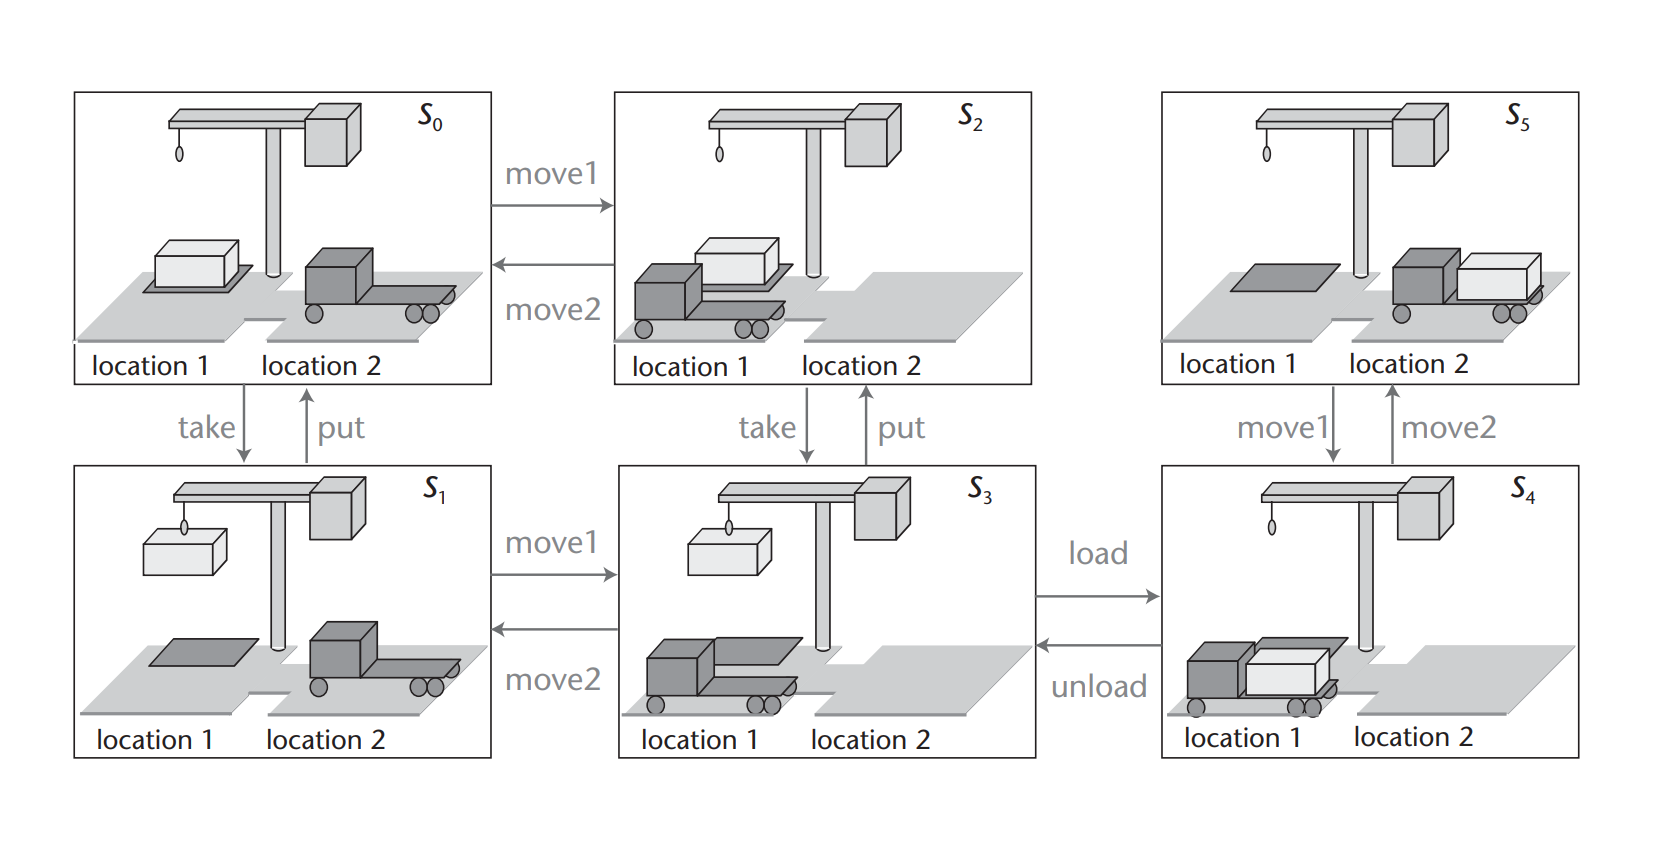
\includegraphics[width=1\linewidth]{figures/state-transition-example.png}
  \caption{A State-Transition System for a Simple Domain Involving a Crane and a
    Robot for Transporting Containers}
  \label{fig:state-transition-diagram}
\end{figure}

\section{Planners}
The planner's input is a \textit{planning problem}, which includes a description
of the system $\sum$, an initial situation and some objective. For example, in
figure \ref{fig:state-transition-diagram}, a planning problem $P$ might consist
of a description of $\sum$, the initial state $s_0$, and a single goal state
$s_5$.

The planner's output is a plan or policy that solves the planning problem. A
\textit{plan} is a sequence of actions such as

\begin{sspara}
$<$take, move1, load, move2$>$.
\end{sspara}

A \textit{policy} is a partial function from states into actions, such as

\begin{sspara}
$\{(s_0, take), (s_1, move1), (s_3, load), (s_4, move2)\}$.
\end{sspara}

The aforementioned plan and policy both solve the planning problem P. Either of
them, if executed starting at the initial state $s_0$, will take $\sum$ through
the sequence of states $\langle s1, s2, s3, s4, s5 \rangle$.

In general, the planner will produce actions that are described at an abstract
level. Hence it may be impossible to perform these actions without first
deciding some of the details. In many planning problems, some of these details
include what resources to use and what time to do the action.

\textit{What Resources to Use}. Exactly what is meant by a \textit{resource}
depends on how the problem is specified. For example, if $\sum$ contained more
than one robot, then one approach would be to require the robot's name as part
of the action (for example, \textsf{move1(robot)} and \textsf{move1(robot2))},
and another approach would be to consider the robot to be a resource whose
identity will be determined later.

\textit{What Time to Do the Action}. For example, in order to load the container
onto the robot, we might want to start moving the crane before the robot arrives
at \textsf{location1}, but we cannot complete the load operation until after the
robot has reached \textsf{location1} and has stopped moving.

In such cases, one approach is to have a separate program called a
\textit{scheduler} that sits in between the planner and the controller (see
figure \ref{fig:planner-diagram}c), whose purpose is to determine those
details. Another approach is to integrate the scheduling function directly into
the planner. The latter approach can substantially increase the complexity of
the planner, but on complex problems it can be much more efficient than having a
separate scheduler.

\section{Controllers}

The \textit{controller}'s input consists of plans (or schedules, if the system
includes a scheduler) and observations about the current state of the system.
The controller's output consists of actions to be performed in the
state-transition system.

In figure \ref{fig:planner-diagram}, notice that the controller is
\textit{online}. As it performs its actions, it receives \textit{observations},
each observation being a collection of sensor inputs giving information about
$\sum$'s current state. The observations can be modeled as an observation
function $\eta : S \rightarrow O$ that maps $S$ into some discrete set of
possible observations. Thus, the input to the controller is the observation $o =
\eta(s)$, where $s$ is the current state.

If $\eta$ is a one-to-one function, then from each observation $o$ we can deduce
exactly what state $\sum$ is in. In this case we say that the observations
provide \textit{complete} information. For example, in figure
\ref{fig:state-transition-diagram}, if there were a collection of sensors that
always provided the exact locations of the robot and the container, then this
sensor would provide complete information—or, at least, complete information for
the level of abstraction used in the figure.

If $\eta$ is not a one-to-one function, then the best we can deduce from an
observation $o$ is that $\sum$ is in one of the states in the set $\eta_{-1}(o)
\subseteq S$, and in this case we say that the observations provide
\textit{incomplete} information about $\sum$’s current state. For example, in
figure \ref{fig:state-transition-diagram}, if we had a sensor that told us the
location of the robot but not the location of the container, this sensor would
provide incomplete information.

\section{Assumptions in Classical Planning}
\label{appendix:assumptions}
\cite{Nau2007} also describes a set of assumptions that classical planners make
about the domain they will work on:

\paragraph*{\textit{Assumption A0 (Finite $\sum$).}} The system $\sum$ has a
finite set of states.

\paragraph*{\textit{Assumption A1 (Fully Observable $\sum$).}} The system $\sum$
is \textit{fully observable}, that is, one has complete knowledge about the
state of $\sum$; in this case the observation function $\eta$ is the identity
function.

\paragraph*{\textit{Assumption A2 (Deterministic $\sum$).}} The system $\sum$ is
\textit{deterministic}, that is, for every state $s$ and event or action $u$,
$|\gamma(s, u)| \leq 1$. If an action is applicable to a state, its application
brings a deterministic system to a single other state. Similarly for the
occurrence of a possible event.

\paragraph*{\textit{Assumption A3 (Static $\sum$).}} The system $\sum$ is
\textit{static}, that is, the set of events $E$ is empty. $\sum$ has no internal
dynamics; it stays in the same state until the controller applies some action.

\paragraph*{\textit{Assumption A4 (Attainment Goals).}} The only kind of goal is
an \textit{attainment goal}, which is specified as an explicit goal state or a
set of goal states $S_g$. The objective is to find any sequence of state
transitions that ends at one of the goal states. This assumption excludes, for
example, states to be avoided, constraints on state trajectories, and utility
functions.

\paragraph*{\textit{Assumption A5 (Sequential Plans).}} A solution plan to a
planning problem is a linearly ordered finite sequence of actions.

\paragraph*{\textit{Assumption A6 (Implicit Time).}} Actions and events have no
duration, they are instantaneous state transitions. This assumption is embedded
in the state-transition model, which does not represent time explicitly.

\paragraph*{\textit{Assumption A7 (Off-line Planning).}} The planner is not
concerned with any change that may occur in $\sum$ \textit{while} it is
planning; it plans for the given initial and goal states regardless of the
current dynamics, if any.

%%% Local Variables:
%%% mode: latex
%%% TeX-master: "../diss"
%%% End:

  %\chapter{Code}
  %\section{core.clj}
\begin{lstlisting}
(ns bitmaid.core
  (:gen-class)
  (:require [bitmaid.domain.compiler :as c]
            [bitmaid.domain.executor :as e]
            [bitmaid.jshop-wrapper :refer :all]
            [clojure.java.shell :refer [sh]]
            [clojure.pprint :refer [pprint]]))

(defn re-files
  ([re]
   (re-files re "."))
  ([re dir]
   (let [files (->> (clojure.java.io/file dir)
                    (.listFiles)
                    (filter #(.isFile %))
                    (filter #(re-matches re (.getName %))))]
     (if (empty? files)
       nil
       files))))

(defn delete-files
  [files]
  (doseq [f files]
    (clojure.java.io/delete-file f)))

(defn generate-plan
  [domain problem]
  (println "Create domain file")
  (spit "housedomain" (with-out-str (pprint (e/encode domain))))

  (println "Create problem file")
  (spit "problem" (with-out-str (pprint (e/encode problem))))

  (println "Compile domain")
  (gen-domain "housedomain")

  (println "Compile problem")
  (gen-plan "problem")

  (println "Recompile problem")
  (sh "javac"
      "-classpath" ".:resources/JSHOP2.jar:resources/antlr.jar"
      "problem.java")

  (println "Plan")
  (let [plan (sh "java"
                 "-classpath" ".:resources/JSHOP2.jar"
                 "problem")]

    (println "Delete class files")
    (delete-files (re-files #".*\.class"))

    (println "Delete java files")
    (delete-files (re-files #".*\.java"))

    (println "Delete domain files")
    (delete-files (re-files #"housedomain.*"))

    (println "Delete problem file")
    (delete-files (re-files #"problem"))

    (println "Shutting down agents")
    (shutdown-agents)

    (println "Finished")
    (parse-plan-text (:out plan))))

(defn file->dom-ext
  [file]
  (-> file
      (slurp)
      (c/precompile-domain-extension)))

(defn file->problem
  [file]
  (-> file
      (slurp)
      (c/precompile-problem)))

(defn extend-domain
  [base extension]
  (-> base
      (update :axioms (partial merge (:axioms extension)))
      (update :methods (partial merge (:methods extension)))
      (update :operators (partial merge (:operators extension)))))

(comment
  (def domain
    (->> (re-files #".*\.dext")
         (map file->dom-ext)
         (reduce (fn
                   ([] nil)
                   ([& args] (apply extend-domain args))))))

  (def problem
    (->> (re-files #".*\.prob")
         (first)
         (file->problem))))

(defn -main
  [& args]
  (println "Searching for domain extension files")
  (if-let [domain-files (re-files #".*\.dext")]
    (do
      (println "Found domain extensions:")
      (doseq [f domain-files]
        (println (.getName f)))

      (if-let [problem-files (re-files #".*\.prob")]
        (let [problem-file (first problem-files)]
          (println "Found a problem file:")
          (println (.getName problem-file))

          (println "Compiling domain extensions")
          (if-let [domain (some->> domain-files
                                   (map file->dom-ext)
                                   (reduce (fn
                                             ([] nil)
                                             ([& args] (apply extend-domain args)))))]
            (do
              (println "Compiling problem")
              (if-let [problem (file->problem problem-file)]
                (do
                  (println "Generating plan")
                  (if-let [plan (generate-plan domain problem)]
                    (do
                      (println)
                      (println "Plan found!")
                      (println (str "Plan: " (:plan plan)))
                      (println (str "Cost: " (:cost plan))))
                    (do
                      (println)
                      (println "No plans were found"))))
                (println "Failed to compile problem")))
            (println "Failed to compile domain extensions")))
        (println "No problem file found")))
    (println "No domain extensions found")))
\end{lstlisting}

\section{Parser - parser.clj}
\begin{lstlisting}
(ns bitmaid.domain.parser
  (:require [clojure.spec.alpha :as s]
            [clojure.spec.gen.alpha :as gen]
            [clojure.set :refer [union subset?]]
            [expound.alpha :refer [expound]]))

(s/def ::variable-symbol
  (s/and symbol?
         (comp #{\?} first name)))

(s/def ::task-symbol
  (s/and symbol?
         (comp #{\!} first name)))

(def restricted-symbols
  #{'not 'call 'and 'or 'imply 'forall 'def})

(defn restricted?
  [symbol]
  (boolean (restricted-symbols symbol)))

(s/def ::general-symbol
  (s/and (some-fn keyword? symbol?)
         (comp not #{\? \!} first name)
         (comp not restricted?)))

(s/def ::constant-symbol ::general-symbol)
(s/def ::predicate-symbol ::general-symbol)
(s/def ::compound-task-symbol ::general-symbol)

(s/def ::function-symbol ::general-symbol)

(s/def ::list nil)
(s/def ::call nil)

(s/def ::term
  (s/or
   :variable-symbol ::variable-symbol
   :constant-symbol ::constant-symbol
   :number   number?
   :call     ::call
   :list     ::list))

(s/def ::list
  (s/and vector?
         (s/coll-of ::term)))

(s/def ::call
  (s/and list?
         (s/cat :call #{'call}
                :function-symbol ::function-symbol
                :terms (s/* ::term))))

(s/def ::logical-atom*
  (s/and list?
       (s/cat :predicate-symbol ::predicate-symbol
              :terms (s/* ::term))))

(s/def ::logical-atom
  (s/or :late-binding ::variable-symbol
        :logical-atom ::logical-atom*))

(s/def ::conjunction nil)
(s/def ::disjunction nil)
(s/def ::negation nil)
(s/def ::implication nil)
(s/def ::universal-quantification nil)
(s/def ::assignment nil)

(s/def ::expression
  (s/or :conjunction  ::conjunction
        :disjunction  ::disjunction
        :negation     ::negation
        :implication  ::implication
        :universal-quantification ::universal-quantification
        :assignment   ::assignment
        :call         ::call
        :logical-atom ::logical-atom))

(s/def ::conjunction
  (s/or :empty (every-pred list? empty?)
        :normal (s/cat :and #{'and}
                       :expressions (s/* ::expression))))

(s/def ::disjunction
  (s/cat :or #{'or}
         :expressions (s/* ::expression)))

(s/def ::negation
  (s/cat :not #{'not}
         :expression ::expression))

(s/def ::implication
  (s/cat :imply #{'imply}
         :lhs ::expression
         :rhs ::expression))

(defn walk-tree
  "Returns a sequence of the nodes in a tree, via depth-first walk."
  [tree]
  (tree-seq seqable? identity tree))

(defn find-variables
  "Returns a set of the variables found in a spec form."
  [spec-form]
  (->> (walk-tree spec-form)
       (filter #(and (seqable? %)
                     (= :variable-symbol (first %))))
       (map second)
       set))

(defn set=
  "Returns true if all vectors input contain the same elements."
  [& vectors]
  (apply = (map set vectors)))

(s/def ::universal-quantification
  (s/and
   (s/cat :forall #{'forall}
          :variable-symbols (s/and vector?
                                   (s/coll-of ::variable-symbol))
          :predicate ::expression
          :form ::expression)
   (fn [form]
     (let [predicate (:predicate form)]
       (if (and (= :logical-atom (first predicate))
                (= :late-binding (first (second predicate))))
         true
         (let [vars (:variable-symbols form)]
           (set= vars (find-variables predicate))))))))

(s/def ::assignment
  (s/cat :def #{'def}
         :name ::variable-symbol
         :value ::term))

(s/def ::first-satisfier-precondition
  (s/cat :first #{:first}
         :expression ::expression))

(s/def ::sorted-precondition
  (s/cat :first #{:sort-by}
         :variable-symbol ::variable-symbol
         :comparator ::function-symbol
         :expression ::expression))

(s/def ::logical-precondition
  (s/or :first-satisfier-precondition ::first-satisfier-precondition
        :sorted-precondition ::sorted-precondition
        :expression ::expression))

(s/def ::axiom
  (s/cat :axiom #{':-}
         :head ::logical-atom
         :axioms (s/* (s/alt :named (s/cat :name ::general-symbol
                                           :logical-precondition ::logical-precondition)
                             :unnamed (s/cat :logical-precondition ::logical-precondition)))))

(s/def ::normal-task-atom
  (s/cat :name ::task-symbol
         :terms (s/* ::term)))

(s/def ::normal-compound-task-atom
  (s/cat :name ::compound-task-symbol
         :terms (s/* ::term)))

(s/def ::task-atom*
  (s/alt :primitive ::normal-task-atom
         :compound ::normal-compound-task-atom))

(s/def ::task-atom
  (s/or :immediate-task (s/cat :immediate #{':immediate}
                               :task ::task-atom*)
        :normal-task ::task-atom*))

(s/def ::task-list nil)

(s/def ::task-list-element
  (s/or :task-atom ::task-atom
        :task-list ::task-list))

(s/def ::task-list*
  (s/* ::task-list-element))

(s/def ::task-list
  (s/and vector?
         (s/alt :unordered (s/cat :unordered #{':unordered}
                                  :task-lists ::task-list*)
                :ordered (s/cat :task-lists ::task-list*))))

(s/def ::protection-condition
  (s/cat :protection #{':protection}
         :logical-atom ::logical-atom))

(s/def ::forall-expression
  (s/and
   (s/cat :forall #{'forall}
          :variable-symbols (s/and vector?
                                   (s/coll-of ::variable-symbol))
          :predicate ::expression
          :logical-atoms (s/and vector?
                                (s/coll-of ::logical-atom*)))))

(s/def ::delete-add-element
  (s/or :logical-atom ::logical-atom
        :protection-condition ::protection-condition
        :forall-expresssion ::forall-expression))

(s/def ::delete-add-list*
  (s/and vector?
         (s/coll-of ::delete-add-element)))

(s/def ::delete-add-list
  (s/or :late-binding ::variable-symbol
        :delete-add-list ::delete-add-list*))

(s/def ::operator
  (s/&
   (s/alt :set-cost (s/cat :operator #{':operator}
                           :head (s/or :normal-task ::normal-task-atom)
                           :precondition ::logical-precondition
                           :delete-list ::delete-add-list
                           :add-list ::delete-add-list
                           :cost number?)
          :no-cost  (s/cat :operator #{':operator}
                           :head (s/or :normal-task ::normal-task-atom)
                           :precondition ::logical-precondition
                           :delete-list ::delete-add-list
                           :add-list ::delete-add-list))))

(s/def ::method
  (s/cat :method #{':method}
         :head (s/or :compound-task ::normal-compound-task-atom)
         :options (s/* (s/alt :named (s/cat :name ::general-symbol
                                            :precondition ::logical-precondition
                                            :tail ::task-list)
                              :unnamed (s/cat :precondition ::logical-precondition
                                              :tail ::task-list)))))

(s/def ::domain-extension
  (s/coll-of (s/alt :method ::method
                    :operator ::operator
                    :axiom ::axiom)))

(def ground? (comp empty? find-variables))

(s/def ::state-list
  (s/and vector?
         (s/* ::logical-atom*)))

(s/def ::problem
  (s/&
   (s/cat :defproblem #{'defproblem}
          :initial-state ::state-list
          :task-list ::task-list)
   (comp ground? :initial-state)))

(defn parse-spec
  "Takes a spec and a form to be parsed or a string containing a form to be parsed,
  attempts to parse it.
  If the form is invalid of produces and error while parsing, returns nil."
  [spec form]
  (try
    (let [form (if (string? form) (read-string form) form)
          parsed (s/conform spec form)]
      (if (not (= :clojure.spec.alpha/invalid parsed))
        parsed
        (do
          (println "Failed to parse input form.")
          (expound spec form))))
    (catch Exception e (println "Parsing form caused an exception."))))


(defn parse-domain-extension
  "Takes a `domain-extension` form, or a string containing the form, and attempts to parse it.
  If the form is invalid or produces an error while parsing returns nil."
  [form]
  (parse-spec ::domain-extension form))

(defn parse-problem
  "Takes a `problem` form, or a string containing the form, and attempts to parse it.
  If the form is invalid or produces an error while parsing returns nil."
  [form]
  (parse-spec ::problem form))
\end{lstlisting}

\section{Pre-compiler - compiler.clj}
\begin{lstlisting}
(ns bitmaid.domain.compiler
  (:require [bitmaid.domain.parser :as p]
            [clojure.spec.alpha :as s]))

;; Utils
(def gen-debug-name gensym)
(defn list-args
  "Given a spec form, return a vector of the variables found."
  [spec-form]
  (->> (p/walk-tree spec-form)
       (filter #(and (seqable? %)
                     (= :variable-symbol (first %))))
       (map second)))

;; Compiler
(defrecord Variable [name])
(defrecord Constant [name])
(defrecord TermNumber [value])

(defrecord Call [function-symbol args])
(def compile-term nil)
(defn compile-call
  [call]
  (map->Call {:function-symbol (:function-symbol call)
              :args (map compile-term (:terms call))}))


(defrecord TermList [values])
(defn compile-list
  [list]
  (map->TermList {:values (map compile-term list)}))

(defn compile-term
  [term]
  (let [type (first term)
        body (second term)]
    (case type
      :variable-symbol (map->Variable {:name body})
      :constant-symbol (map->Constant {:name body})
      :number (map->TermNumber {:value body})
      :call (compile-call body)
      :list (compile-list body))))

(def compile-expression nil)
(defrecord Conjunction [expressions])
(defn compile-conjunction
  [con]
  (let [empty? (= :empty (first con))
        body (second con)
        expressions (if empty?
                      []
                      (:expressions body))]
    (map->Conjunction {:expressions (map compile-expression expressions)})))

(defrecord Disjunction [expressions])
(defn compile-disjunction
  [dis]
  (map->Disjunction {:expressions (map compile-expression (:expressions dis))}))

(defrecord Negation [expression])
(defn compile-negation
  [neg]
  (map->Negation {:expression (compile-expression (:expression neg))}))

(defrecord Implication [lhs rhs])
(defn compile-implication
  [implication]
  (map->Implication {:lhs (compile-expression (:lhs implication))
                     :rhs (compile-expression (:rhs implication))}))

(defrecord UniversalQuantification [variables predicate form])
(defn compile-universal-quantification
  [quantif]
  (map->UniversalQuantification {:variables (:variable-symbols quantif)
                                 :predicate (compile-expression (:predicate quantif))
                                 :form (compile-expression (:form quantif))}))

(defrecord Assignment [name value])
(defn compile-assignment
  [assignment]
  (map->Assignment {:name (:name assignment)
                    :value (compile-term (:value assignment))}))

(defrecord LateBinding [name])
(defrecord LogicalAtom [name args])
(defn compile-base-logical-atom
  [atom]
  (let [name (:predicate-symbol atom)]
    (map->LogicalAtom {:name name
                       :args (map compile-term (:terms atom))})))
(defn compile-logical-atom
  [atom]
  (let [late-binding? (= :late-binding (first atom))
        body (second atom)]
    (if late-binding?
      (map->LateBinding {:name body})
      (compile-base-logical-atom body))))

(defn compile-expression
  [expression]
  (let [type (first expression)
        body (second expression)]
    (case type
      :conjunction  (compile-conjunction body)
      :disjunction  (compile-disjunction body)
      :negation     (compile-negation body)
      :implication  (compile-implication body)
      :universal-quantification (compile-universal-quantification body)
      :assignment   (compile-assignment body)
      :call         (compile-call body)
      :logical-atom (compile-logical-atom body))))

(defrecord FirstSatisfierPrecondition [expression])
(defn compile-first-satisfier-precondition
  [precond]
  (map->FirstSatisfierPrecondition {:expression (compile-expression (:expression precond))}))

(defrecord SortedPrecondition [variable comparator expression])
(defn compile-sorted-precondition
  [precond]
  (map->SortedPrecondition {:variable (:variable-symbol precond)
                            :comparator (:comparator precond)
                            :expression (compile-expression (:expression precond))}))

(defn compile-logical-precondition
  [precond]
  (let [type (first precond)
        body (second precond)]
    (case type
      :first-satisfier-precondition (compile-first-satisfier-precondition body)
      :sorted-precondition (compile-sorted-precondition body)
      :expression (compile-expression body))))

(defrecord TaskAtom [name args immediate? primitive?])
(defn compile-task-atom
  [atom]
  (let [immediate? (= :immediate-task (first atom))
        body (if immediate?
               (:task (second atom))
               (second atom))
        primitive? (= :primitive (first body))
        body (second body)
        name (:name body)
        args (map compile-term (:terms body))]
    (map->TaskAtom {:name name
                    :args args
                    :immediate? immediate?
                    :primitive? primitive?})))

(defrecord TaskList [task-lists ordered?])
(def compile-task-list nil)
(defn compile-task-list*
  [list]
  (let [task-atom? (= :task-atom (first list))
        body (second list)]
    (if task-atom?
      (compile-task-atom body)
      (compile-task-list body))))

(defn compile-task-list
  [list]
  (let [ordered? (= :ordered (first list))
        body (second list)]
    (map->TaskList {:task-lists (map compile-task-list* (:task-lists body))
                    :ordered? ordered?})))

(defrecord MethodOption [name precondition tail])
(defn compile-method-option
  [option]
  (let [named? (= :named (first option))
        body (second option)
        name (if named?
               (:name body)
               (gen-debug-name "method-branch_"))
        precondition (compile-logical-precondition (:precondition body))
        tail (compile-task-list (:tail body))]
    (map->MethodOption {:name name
                        :precondition precondition
                        :tail tail})))

(defrecord Method [name args options])
(defn method-name
  [method]
  (-> method
      :head
      second
      :name))

(defn compile-method
  [method]
  (let [name (method-name method)
        args (list-args (:head method))
        options (map compile-method-option (:options method))]
    (map->Method {:name name
                  :args args
                  :options options})))

(defrecord ProtectionCondition [atom])
(defn compile-protection-condition
  [protec]
  (map->ProtectionCondition {:atom (compile-logical-atom (:logical-atom protec))}))

(defrecord ForallExpression [variables predicate logical-atoms])
(defn compile-forall-expression
  [forall]
  (map->ForallExpression {:variables (:variable-symbols forall)
                          :predicate (compile-expression (:predicate forall))
                          :form (map compile-logical-atom (:logical-atoms forall))}))

(defn compile-delete-add-element
  [element]
  (let [type (first element)
        body (second element)]
    (case type
      :logical-atom (compile-logical-atom body)
      :protection-condition (compile-protection-condition body)
      :forall-expresssion (compile-forall-expression body))))

(defn compile-delete-add-list
  [list]
  (let [late-binding? (= :late-binding (first list))
        body (second list)]
    (if late-binding?
      (map->LateBinding {:name body})
      (map compile-delete-add-element body))))

(defn operator-name
  [operator]
  (-> operator
      second
      :head
      second
      :name))

(defrecord Operator [name args precondition delete-list add-list cost])
(defn compile-operator
  [operator]
  (let [has-cost? (= :set-cost (first operator))
        body (second operator)
        cost (if has-cost?
               (:cost body)
               1)
        name (operator-name operator)
        args (list-args (:head body))
        precondition (compile-logical-precondition (:precondition body))
        delete-list (compile-delete-add-list (:delete-list body))
        add-list (compile-delete-add-list (:add-list body))]
    (map->Operator {:name name
                    :args args
                    :precondition precondition
                    :delete-list delete-list
                    :add-list add-list
                    :cost cost})))

(defrecord AxiomPrecondition [name precondition])
(defn compile-axiom-precondition
  [precondition]
  (let [named? (= :named (first precondition))
        body (second precondition)
        name (if named?
               (:name body)
               (gen-debug-name "axiom-precondition_"))]
    (map->AxiomPrecondition {:name name
                             :precondition (compile-logical-precondition (:logical-precondition body))})))

(defn axiom-name
  [axiom]
  (-> axiom
      :head
      second
      :predicate-symbol))

(defrecord Axiom [name args preconditions])
(defn compile-axiom
  [axiom]
  (map->Axiom {:name (axiom-name axiom)
               :args (list-args (:head axiom))
               :preconditions (map compile-axiom-precondition (:axioms axiom))}))


(defrecord DomainExtension [methods operators axioms])
(defn compile-domain-extension
  [domain-extension]
  (loop [acc domain-extension
         methods {}
         operators {}
         axioms {}]
    (if (empty? acc)
      (map->DomainExtension {:methods methods
                             :operators operators
                             :axioms axioms})
      (let [next (first acc)
            type (first next)
            body (second next)]
        (case type
          :method (recur (rest acc)
                         (assoc methods (method-name body) (compile-method body))
                         operators
                         axioms)
          :operator (recur (rest acc)
                           methods
                           (assoc operators (operator-name body) (compile-operator body))
                           axioms)
          :axiom (recur (rest acc)
                        methods
                        operators
                        (assoc axioms (axiom-name body) (compile-axiom body))))))))

(defrecord Problem [initial-state task-list])
(defn compile-problem
  [problem]
  (let [initial-state (map compile-base-logical-atom (:initial-state problem))
        task-list (compile-task-list (:task-list problem))]
    (map->Problem {:initial-state initial-state
                   :task-list task-list})))

(defn precompile-domain-extension
  [domain-extension]
  (compile-domain-extension
   (p/parse-domain-extension domain-extension)))

(defn precompile-problem
  [problem]
  (compile-problem
   (p/parse-problem problem)))
\end{lstlisting}

\section{Encoder - executor.clj}
\begin{lstlisting}
(ns bitmaid.domain.executor
  (:require [bitmaid.domain.compiler :as c]
            [bitmaid.domain.parser :as p]
            [clojure.spec.alpha :as s])
  ;; Import records
  (:import [bitmaid.domain.compiler Variable
            Constant TermNumber Call TermList
            Conjunction Disjunction Negation
            Implication UniversalQuantification
            Assignment LateBinding LogicalAtom
            FirstSatisfierPrecondition SortedPrecondition
            TaskAtom TaskList MethodOption
            Method ProtectionCondition ForallExpression
            Operator AxiomPrecondition Axiom DomainExtension
            Problem]))

(def flatten-1 (partial mapcat identity))

(defprotocol JSHOPEncode
  (encode [this] "Encode the given form into a form that the JSHOP compiler will understand."))

(extend-protocol JSHOPEncode
  Variable
  (encode
    [{:keys [name]}]
    name)
  Constant
  (encode
    [{:keys [name]}]
    name)
  TermNumber
  (encode
    [{:keys [value]}]
    value)
  Call
  (encode
    [{:keys [function-symbol args]}]
    `(~'call ~function-symbol ~@(map encode args)))
  TermList
  (encode
    [{:keys [values]}]
    `(~@(map encode values)))
  Conjunction
  (encode
    [{:keys [expressions]}]
    (if (empty? expressions)
      `()
      `(~'and ~@(map encode expressions))))
  Disjunction
  (encode
    [{:keys [expressions]}]
    `(~'or ~@(map encode expressions)))
  Negation
  (encode
    [{:keys [expression]}]
    `(~'not ~(encode expression)))
  Implication
  (encode
    [{:keys [lhs rhs]}]
    `(~'imply ~(encode lhs) ~(encode rhs)))
  UniversalQuantification
  (encode
    [{:keys [variables predicate form]}]
    `(~'forall (~@variables)
               ~(encode predicate)
               ~(encode form)))
  Assignment
  (encode
    [{:keys [name value]}]
    `(~'assign ~name ~(encode value)))
  LateBinding
  (encode
    [{:keys [name]}]
    name)
  LogicalAtom
  (encode
    [{:keys [name args]}]
    `(~name ~@(map encode args)))
  FirstSatisfierPrecondition
  (encode
    [{:keys [expression]}]
    `(~':first ~(encode expression)))
  SortedPrecondition
  (encode
    [{:keys [variable comparator expression]}]
    `(~':sort-by ~variable ~comparator ~(encode expression)))
  TaskAtom
  (encode
    [{:keys [name args immediate? primitive?]}]
    `(~@(when immediate? [':immediate])
      ~name
      ~@(map encode args)))
  TaskList
  (encode
    [{:keys [task-lists ordered?]}]
    `(~@(when (not ordered?) [':unordered])
      ~@(map encode task-lists)))
  MethodOption
  (encode
    [{:keys [name precondition tail]}]
    `(~name
      ~(encode precondition)
      ~(encode tail)))
  Method
  (encode
    [{:keys [name args options]}]
    `(~':method (~name ~@args)
      ~@(flatten-1 (map encode options))))
  ProtectionCondition
  (encode
    [{:keys [atom]}]
    `(~':protection ~(encode atom)))
  ForallExpression
  (encode
    [{:keys [variables predicate logical-atoms]}]
    `(~'forall (~@variables)
      ~(encode predicate)
      (~@(map encode logical-atoms))))
  Operator
  (encode
    [{:keys [name args precondition delete-list add-list cost]}]
    `(~':operator (~name ~@args)
      ~(encode precondition)
      (~@(map encode delete-list))
      (~@(map encode add-list))
      ~cost))
  AxiomPrecondition
  (encode
    [{:keys [name precondition]}]
    `(~name
      ~(encode precondition)))
  Axiom
  (encode
    [{:keys [name args preconditions]}]
    `(~':- (~name ~@args)
      ~@(flatten-1 (map encode preconditions))))
  DomainExtension
  (encode
    [{:keys [axioms methods operators]}]
    `(~'defdomain ~'housedomain
      (~@(->> (list axioms methods operators)
              (map vals)
              (flatten-1)
              (map encode)))))
  Problem
  (encode
    [{:keys [initial-state task-list]}]
    `(~'defproblem ~'problem ~'housedomain
       (~@(map encode initial-state))
       (~@(encode task-list)))))
\end{lstlisting}

%%% Local Variables:
%%% mode: latex
%%% TeX-master: "../diss"
%%% End:

  \chapter{Simple Home Example}
  \label{appendix:home-example}
  \section{Problem File - p.prob}
This problem file describes a home with several lights in it as well as the
current hour of the day. The problem also specifies to run the `automate-house'
method first, this is where the user defined rules are.

\begin{lstlisting}
(defproblem
  [(hour 12)
   (light light1) (on light1)
   (light light2) (off light2)
   (light light3) (on light3)
   (light light4) (off light4)
   (light light5) (off light5)
   (light light6) (on light6)
   (light light7) (off light7)
   (light light8) (off light8)
   (light light9) (on light9)]
  [(automate-house)])
\end{lstlisting}

\section{User Defined rules - user-rules.dext}
This domain extension describes the rules that the manager would have configured
in the home automation system's user interface. In this case the rules are: if
it is the afternoon and there are some lights on, then turn all the lights off;
and if it is the morning or the evening and there are some lights off, then turn
all the lights on.

\begin{lstlisting}
[(:method (rule-1)
          (and (afternoon)
               (not
                (forall [?light]
                        (light ?light)
                        (off ?light))))
          [(!turn-off-all)]
          ()
          [])

 (:method (rule-2)
          (and (or (evening)
                   (morning))
               (not
                (forall [?light]
                        (light ?light)
                        (on ?light))))
          [(!turn-on-all)]
          ()
          [])

 (:method (automate-house)
          ()
          [(rule-1) (rule-2)])]
\end{lstlisting}

\section{Time Middleware - time.dext}
This domain extension describes a simple example of a middleware that provides
three axiom predicates for describing the time of day.

\begin{lstlisting}
[(:- (morning)
     (and (hour ?hour)
          (call > ?hour 0)
          (call < ?hour 6)))

 (:- (afternoon)
     (and (hour ?hour)
          (call >= ?hour 6)
          (call < ?hour 20)))

 (:- (evening)
     (and (hour ?hour)
          (call >= ?hour 20)
          (call < ?hour 24)))]
\end{lstlisting}

\section{Device Driver - light1.dext}
This domain extension describes a simple device driver to interface with the
lights configured in the system.

\begin{lstlisting}
[(:operator (!turn-on ?light)
            (and (light ?light)
                 (off ?light))
            [(off ?light)]
            [(on ?light)])

 (:operator (!turn-on-all)
            ()
            [(forall [?light]
                     (and (light ?light)
                          (off ?light))
                     [(off ?light)])]
            [(forall [?light]
                     (and (light ?light)
                          (off ?light))
                     [(on ?light)])])

 (:operator (!turn-off ?light)
            (and (light ?light)
                 (on ?light))
            [(on ?light)]
            [(off ?light)])

 (:operator (!turn-off-all)
            ()
            [(forall [?light]
                     (and (light ?light)
                          (on ?light))
                     [(on ?light)])]
            [(forall [?light]
                     (and (light ?light)
                          (on ?light))
                     [(off ?light)])])

 (:method (toggle-light-internal ?light)
          (on ?light)
          [(!turn-off ?light)]
          (off ?light)
          [(!turn-on ?light)])

 (:method (toggle-light ?light)
          (light ?light)
          [(toggle-light-internal ?light)])]
\end{lstlisting}

%%% Local Variables:
%%% mode: latex
%%% TeX-master: "../diss"
%%% End:

\end{appendices}

\bibliographystyle{agsm}
\bibliography{references}

\end{document}
